%
% Tesi D.S.I. - modello preso da
% Stanford University PhD thesis style -- modifications to the report style
%
%%%%%%%%%%%%%%%%%%%%%%%%%%%%%%%%%%%%%%%%%%%%%%%%%%%%%%%%%
%
%--fix template
\makeatletter
\let\my@xfloat\@xfloat
\makeatother
%--end fix
\documentclass[a4paper,12pt]{report}
%			PREAMBOLO
%
\usepackage[a4paper]{geometry}
\usepackage{amssymb,amsmath,amsthm}
\usepackage{graphicx}
\graphicspath{{./img/}}
\usepackage{url}
\usepackage{hyperref}
\usepackage{epsfig}
\usepackage[italian]{babel}
\usepackage{setspace}
\usepackage{tesi}
%--definizione linguaggio
\usepackage{listings}
\usepackage{color}
\definecolor{dkgreen}{rgb}{0,0.6,0}
\definecolor{gray}{rgb}{0.5,0.5,0.5}
\definecolor{mauve}{rgb}{0.58,0,0.82}

\lstset{frame=tb,
  language=Bash,
  aboveskip=3mm,
  belowskip=3mm,
  showstringspaces=false,
  columns=flexible,
  basicstyle={\small\ttfamily},
  numbers=none,
  numberstyle=\tiny\color{gray},
  keywordstyle=\color{blue},
  commentstyle=\color{dkgreen},
  stringstyle=\color{mauve},
  breaklines=true,
  breakatwhitespace=true,
  tabsize=3
}
%--fine definizione linguaggio

%--fix template
\makeatletter
\def\@xfloat#1[#2]{
	\my@xfloat#1[#2]%
	\def\baselinestretch{1}%
	\@normalsize \normalsize
}
\makeatother
%--end fix

% per le accentate
\usepackage[utf8]{inputenc}
%
\newtheorem{myteor}{Teorema}[section]
%
\newenvironment{teor}{\begin{myteor}\sl}{\end{myteor}}
%
%			TITOLO
%
\begin{document}
\begin{center}

\includegraphics[width=\textwidth]{Logo.jpg}
\title{Realizzazione di una soluzione IAC (Infrastructure As Code) che consenta il rilascio di un'infrastruttura per ambiti DevOps}
\end{center}
\author{\textbf{Roberto Antoniello}}
\dept{Corso di Laurea in Informatica} 
\anno{2022-2023}
\matricola{\textbf{875693}}
\relatore{Prof. Valentina Ciriani}
\correlatore{Mario Petrella}

\beforepreface

\afterpreface
%  
\chapter{Introduzione}
\section{Descrizione del progetto}
Il progetto di tirocinio è stato svolto presso Certimeter s.r.l., un'azienda di consulenza informatica che opera in diversi settori dell'IT(Information Technology) con sede a Torino e Milano. Un dettaglio interessante è dato dalla sua nascita iniziale come spin-off dell'Università degli studi di Torino.\cite{certimeter}\\
Il progetto è consistito nella definizione, rilascio e controllo di un'infrastruttura IAC.\\
Questa piattaforma aveva il vincolo di dover essere rilasciata in automatico attraverso il cloud e avere la capacità di poter ospitare applicazioni a micro servizi. Inoltre doveva essere in grado di integrare e rilasciare le successive modifiche di questi microservizi in automatico senza ausilio di passi manuali.\\
Tutto il lavoro svolto è ruotato attorno a ciò che viene definito come sviluppo DevOps, una metodologia che andremo a spiegare e discutere nei successivi paragrafi. \\
Oltre a ciò, tutto lo sviluppo è stato pensato con l'obiettivo di simulare un'ambiente reale a tutti gli effetti.\\
In questo capitolo introduttivo saranno descritti gli obiettivi formativi e tecnici del progetto, le fasi principali che sono state svolte, oltre a introdurre le metodologie utilizzate dando così una panoramica più ampia sul progetto e sui concetti che sono stati incontrati e approfonditi. 
Verranno anche fatte alcune considerazioni su ciò che può comportare l'uso di determinati strumenti e soluzioni.\\
In questo modo sarà più immediato richiamare alcuni concetti che useremo nei capitoli successivi.

\subsection{Obiettivi formativi}
Gli obiettivi formativi prefissati per questo progetto di tirocinio sono stati i seguenti:\\
\begin{enumerate}
\item \textit{Acquisire competenze in ambito DevOps.}
\item \textit{Acquisire conoscenze sul ciclo di vita di un'infrastruttura.}\\
Si intende con ciclo di vita che l'obiettivo specifico fosse quello di comprendere e acquisire competenze a partire dall'analisi dei requisiti, per passare poi alla progettazione delle specifiche necessarie fino ad arrivare all'implementazione finale del sistema.\\
Difatti il progetto di tirocinio è stato diviso in diverse fasi ben distinte che comprendono tutte queste caratteristiche.
\end{enumerate}
\subsection{Dal metodo tradizionale all'approccio DevOps}
\textbf{DevOps} è una metodologia che punta a ridurre in modo considerevole i tempi di rilascio di nuovo software incorporando nello stesso di team di sviluppo le competenze necessarie per costruire l'infrastruttura adatta al rilascio del software grazie ai concetti di container, microservizi e cloud computing. Questo fa si che la la collaborazione tra sviluppatori e operatori IT sia molto più stretta e interconnessa. \cite{defdevops}\\
Tradizionalmente il processo di rilascio avveniva più lentamente nell'arco di mesi. Il team di sviluppo doveva coordinarsi con gli altri team per le diverse fasi dello sviluppo. Oggi invece con lo sviluppo DevOps si possono eseguire tutte le fasi senza dover aspettare un team separato, garantendo che il tempo di rilascio delle modifiche del software possa avvenire con frequenza oraria o anche meno, oltre ad essere continuativo e automatico.\\
Un'ulteriore progresso in questo tipo di approcci è il DevSecOps, una strategia che va a integrare anche la sicurezza e il testing nel CI(Continuous Integration) e CD(Continuous Deployment). \\La difficoltà che sorge nel DevSecOps è la risoluzione dei problemi legati alla sicurezza internamente al team di sviluppo, poichè gli sviluppatori devono prima acquisire le competenze necessarie per risolvere questo tipo di problemi.\\

\subsection{Considerazioni}
Nonostante la metodologia appena introdotta e utilizzata nel contesto del progetto risulti molto conveniente, può presentare alcuni svantaggi se analizzata su punti specifici.\\
Ad esempio il \textbf{cloud computing}, strumento di cui parleremo anche più avanti nel capitolo 2, ci permette di avere a disposizione hardware già configurato noleggiato da terzi. Quindi sfruttando le potenzialità della rete non dobbiamo configurarlo in primo luogo noi.\cite{cloud}\\ Dal punto di vista economico è molto vantaggioso siccome il costo è basato solo sul consumo, però ci sarebbe da considerare tutto ciò che riguarda le macchine noleggiate in sè. Essendo già preconfigurate a livello di sistema dall'azienda erogatrice, non abbiamo il potere di personalizzarle appieno e dovremmo accettare questa limitazione con tutte le conseguenze del merito.\\
Per quanto riguarda invece le altre tecnologie che ruotano attorno a \textbf{DevOps}, quelle utilizzate durante il progetto sono state un susseguirsi di alzamento del livello di astrazione man mano che durante la fase di studio si andava al passo successivo.\\
C'è dunque da considerare che al raggiungimento di un certo strato, si possano perdere delle componenti a basso livello essendo implicite in una tecnologia più avanzata e strutturata. Il vantaggio di tutto ciò sta nel dover eseguire meno operazioni per gestire le risorse, esattamente come è avvenuto storicamente nell'evoluzione dei linguaggi di programmazione. D'altro canto, lo svantaggio resta nel minor controllo su determinati elementi che non sono più visibili come in precedenza.


\subsection{Obiettivi tecnici}
Come anticipato, a livello tecnico l'obiettivo principale era di costruire un'infrastruttura in grado di essere rilasciata in automatico attraverso il cloud e sulla quale fosse possibile rilasciare applicazioni basate su microservizi.\\
Per fare ciò sono state sfruttate le conoscenze apprese durante il conseguimento degli obiettivi formativi, con l'utilizzo attivo delle tecnologie studiate alle quali si è dedicato il capitolo successivo.


\section{IAC: definizione e vantaggi}
La metodologia IAC(Infrastructure As Code), in italiano \textit{infrastruttura come codice}, è una strategia che punta a gestire l'intero ciclo di vita di un'infrastruttura mediante codice. Quindi non c'è bisogno di configurazione hardware fisica o strumenti interattivi esterni, è sufficiente uno o più linguaggi dichiarativi o di scripting e compilare correttamente dei file di definizione.\cite{iacdef} \\ 
In questo modo è molto più semplice e rapido modificare o eseguire miglioramenti al sistema senza dover ripensare completamente la struttura o stravolgerne le componenti. \\
Questa metodologia è direttamente relazionata con DevOps poiché gli strumenti che utilizzano IAC puntano a rendere più coesi i team di sviluppo massimizzando la resa finale. L'automazione stessa punta a eliminare tutti quei processi che prima venivano svolti manualmente rendendo tutto lo sviluppo più efficiente e produttivo.\cite{iaceng}\\
Come vedremo nei capitoli successivi, la potenza di alcune delle tecnologie trattate lungo lo sviluppo di questo progetto risiede proprio nel fatto di poter essere gestite direttamente tramite codice.\\ \\ \\ \\ \\ \\

\section{Fasi principali svolte}
Le principali fasi svolte durante il progetto di tirocinio sono state le seguenti:
\begin{enumerate}
\item \textit{Studio delle tecnologie coinvolte.} \\
Durante questa fase sono state approcciate diverse tecnologie per la prima volta. Inizialmente sono stati appresi i concetti a livello teorico che ruotavano attorno al funzionamento di questi strumenti. Successivamente questi concetti sono stati messi in pratica applicandoli a diversi test, partendo da basso livello e salendo man mano di astrazione.\\
\item \textit{Progettazione dell'infrastruttura.} \\
In questa fase è stata eseguita un'analisi dei requisiti e definita la struttura dell'infrastruttura finale. Per fare ciò è stata sfruttata la fase iniziale di studio per capire in che modo le varie tecnologie andassero collegate tra loro correttamente.
\item \textit{Implementazione del sistema.}\\
In questa fase finale è stata implementata l'infrastruttura in funzione dei disegni progettuali prodotti in precedenza.\\
Infine è stata poi rilasciata al suo interno un'applicazione a microservizi. \\
Come da requisiti iniziali anche le successive modifiche all'applicazione potevano avvenire in automatico in regola con la CI/CD. \\
\end{enumerate}
\begin{figure}[h]
	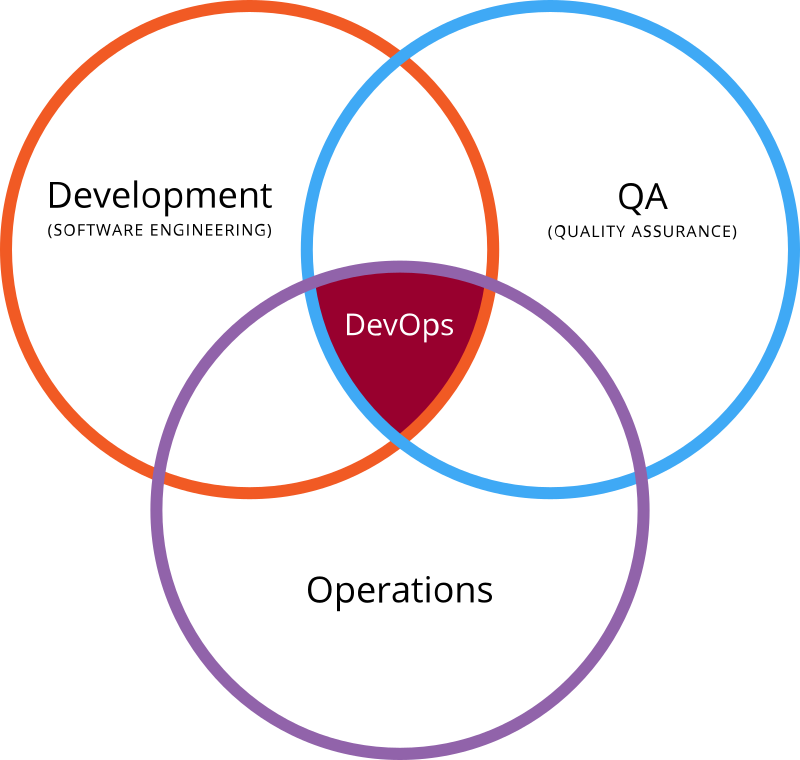
\includegraphics[width=1.0\textwidth]{def_devops}
    \caption{Rappresentazione grafica di come DevOps si ponga nell'intersezione tra sviluppo, garanzia di qualità e operazioni IT.) \cite{defdevops}}
    \label{fig:def_devops}
\end{figure}
%-------------------------------------------------
\chapter{Fase di studio e analisi dei requisiti}
\section{Tecnologie utilizzate}
\begin{figure}[h]
	\centering
	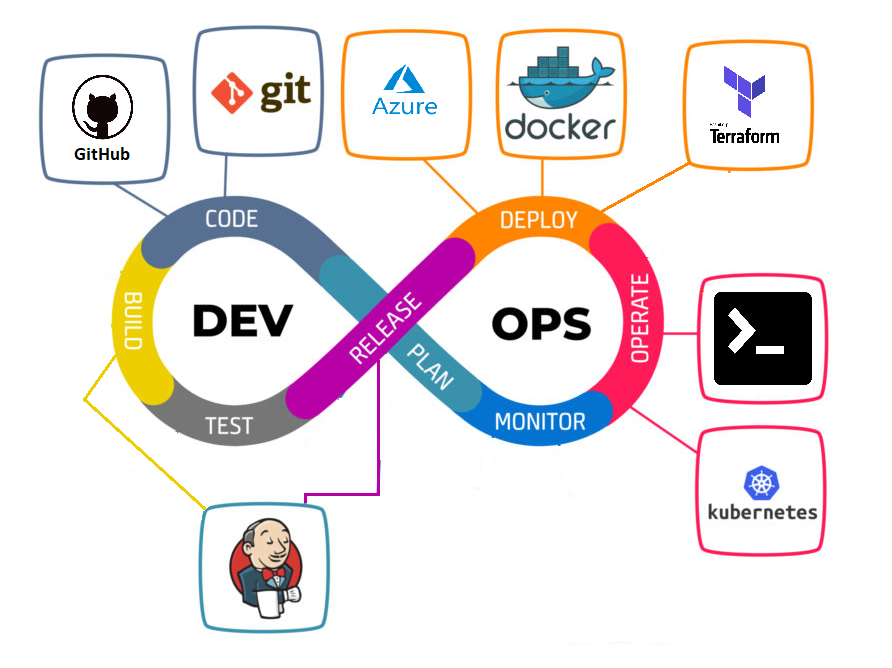
\includegraphics[width=0.6\textwidth]{tech_used}
    \caption{The DevOps infinity loop(ogni tecnologia utilizzata nel proprio settore) \cite{devopsloopimg}}
    \label{fig:tech_used}
\end{figure}
In questa figura è possibile osservare l'elenco delle tecnologie utilizzate, ognuna posta nel proprio settore di appartenenza lungo il ciclo infinito dello sviluppo DevOps.\cite{devopsloop}\\
Questo ciclo parte dalla stesura del codice fino ad arrivare al suo monitoraggio per poi ricominciare da capo senza mai concludersi.\\
Sul settore del deploy notiamo \textbf{Azure} che è il cloud provider scelto durante la fase di studio, \textbf{Terraform} per la vera e propria infrastruttura a livello di codice e \textbf{Docker} per la sua funzionalità nella creazione di container.\\
Potremo invece considerare \textbf{Kubernetes}  come il \textit{'controller'} di tutto il sistema costruito durante il progetto.\\
Infine per la parte di build e release è stato utilizzato \textbf{Jenkins} per tutto ciò che riguarda il continuo rilascio in maniera automatica.\\
Va specificato che l'uso di determinate tecnologie a scapito di altre è legato puramente a vincoli imposti durante il progetto. Il tutto è realizzabile senza problemi utilizzando anche cloud provider diversi o tecnologie con qualità equivalenti per le parti di automazione e rilascio automatico.\\
In questa sezione approfondiremo nel dettaglio le tecnologie menzionate poc'anzi e tutto ciò che è ruotato attorno alla fase di studio. Successivamente rivedremo i requisiti del progetto e come sono state messi insieme i vari strumenti studiati per farli comunicare come un sistema unico.
\subsection{Docker}
Docker è un software progettato per permettere di eseguire applicazioni in ambienti isolati minimali e facilmente distribuibili, anche detti container. \cite{docker} \\
In particolare questi container non sono altro che delle applicazioni "virtualizzate" che condividono il kernel del sistema operativo della macchina che li ospita.\\
Il vantaggio principale nell'utilizzo di Docker risiede nel fatto che sviluppando a piccoli servizi indipendenti rispetto a un'applicazione monolitica tradizionale, nel momento in cui un servizio dovesse andare offline, il resto dell'applicazione sarebbe ancora disponibile. Al contrario con un metodo tradizionale, tutto il sistema crollerebbe in una volta sola.\\
Nel contesto del progetto Docker è stato usato direttamente solo per il versionamento delle immagini dei microservizi. È stato invece usato in modo implicito e indiretto all'interno di Kubernetes. \\ 
\begin{figure}[h]
	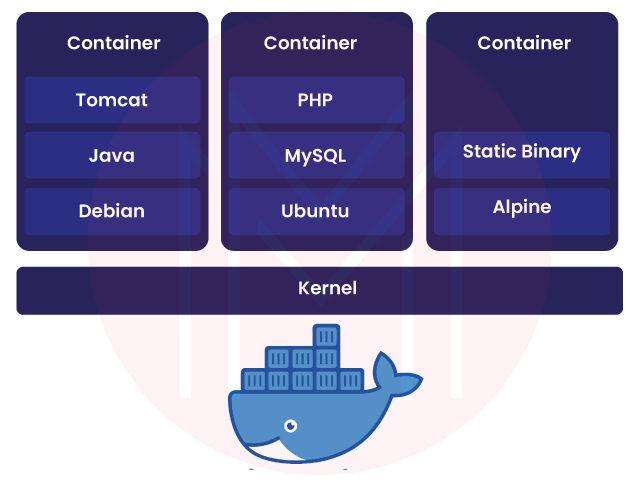
\includegraphics[width=1.0\textwidth]{docker}
    \caption{Esempio di rappresentazione di alcuni container rispetto al kernel del sistema operativo della macchina ospitante. \cite{dockerimg}}
    \label{fig:docker}
\end{figure}
\subsection{Kubernetes}
Kubernetes, anche chiamata k8s, è una piattaforma open source che automatizza le operazioni sui container. Grazie ad essa vengono eliminati molti dei processi manuali coinvolti nel deploy di applicazioni in container. \\
Questa caratteristica viene chiamata orchestrazione, dunque non è più necessario manipolare i container a mano con diversi comandi Docker, ma è sufficiente scrivere un manifesto in codice formato YAML. In questo file vengono definite le specifiche del container e ogni volta che dovrà essere modificato basterà modificare il codice e successivamente applicare di nuovo il file. Il container stesso viene posto all'interno di un oggetto a un livello più alto di atrazione chiamato pod, il quale può essere considerato come una scatola che al suo interno contiene il container e le informazioni che lo definiscono.\\
Questa è una tecnologia che funziona in cluster, quindi ho gruppi di nodi su cui sono in esecuzioni dei container e Kubernetes aiuta a gestirli in modo facile ed efficiente attraverso l'orchestrazione.\\
K8s si pone a un livello d'astrazione più alto rispetto a Docker e i nodi all'interno del cluster contengono già al loro interno un container runtime.\cite{kubernetes}\\ 
Un'ulteriore vantaggio legato a Kubernetes risiede nei suoi meccanismi di autoscale sia orizzontale che verticale oltre che a tecniche di scheduling interne, così da garantire che i servizi delle applicazioni siano sempre disponibili. Dunque, se combinata con il cloud, la potenza di questa tecnologia viene amplificata ulteriormente potendo deployare anche in diverse aree geografiche per minimizzare ancor più la probabilità di avere dei downtime.\\
\begin{figure}[h]
	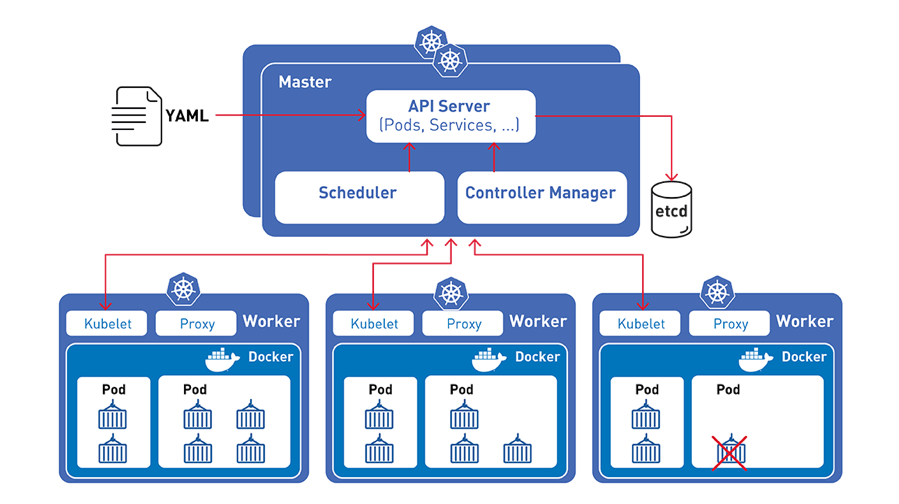
\includegraphics[width=1.0\textwidth]{k8s}
    \caption{Una rappresentazione grafica di un cluster Kubernetes. \cite{k8simg}}
    \label{fig:k8s}
\end{figure}
Ad esempio nella figura 3 si può notare che il cluster è configurato con quattro nodi, uno master e tre worker. All'interno del master vi sono tutte le componenti di sistema di Kubernetes, mentre sui nodi worker risiedono i microservizi deployati. Il contenuto dei manifesti YAML viene comunicato al nodo master che successivamente va a schedulare i container in modo appropriato sui vari nodi.
\subsection{Azure}
Nel corso della fase di studio, tra le varie alternative possibili è stato scelto Azure come cloud provider su cui fare affidamento.\\
I vantaggi di usare il cloud sono molteplici ma quello principale è il non bisogno di costruirsi un proprio datacenter privato acquistando hardware e gestendolo privatamente, ma noleggiandolo da società terze sfruttando la rete.\cite{cloud}\\
L'utilizzo delle macchine è pagato sulla base dell'effettivo consumo e come detto poc'anzi questo fa si che i costi da sostenere siano notevolmente più bassi rispetto all'acquisto, installazione e manutenzione in loco.\\
Nel contesto del progetto Azure è stato usato principalmente per il suo servizio legato ai cluster Kubernetes, chiamato Azure Kubernetes Service o in forma abbreviata AKS. Oltre alla convenienza sul lato economico, un vantaggio in questo caso specifico sta nel ritrovarsi con un cluster già pronto e operativo con un singolo comando dalla CLI di Azure o con pochi click dal portale web.\\
Alternativamente, se dovessimo fare a meno di questo servizio, saremmo costretti a configurare a mano le diverse macchine per collegarle insieme e formare il cluster. Chiaramente vi è anche uno svantaggio legato alla limitazione sulla configurazione dei nodi essendo preimpostati dal servizio di Azure.
\begin{lstlisting}[caption={\\\textit{Esempio di comando per creare un cluster Kubernetes come servizio di Azure da Azure CLI. Gli argomenti passati sono il gruppo risorse in cui deployare la risorsa di tipo AKS, il nome attribuito al cluster e il numero di nodi desiderati.}}]
az aks create \
  --resource-group <gruppo-risorse> \
  --name <nome-cluster> \
  --node-count <n> \
\end{lstlisting}
\subsection{Terraform}
Si tratta di una tecnologia di automazione dotata di un proprio linguaggio dichiarativo HCL(Hashicorp Configuration Language), con la quale è possibile creare, modificare e eventualmente distruggere risorse descritte nel codice.\\
Nel contesto del progetto Terraform è stato utilizzato per definire le specifiche del cluster Kubernetes come servizio di Azure. Una volta che è stato possibile definirlo tramite codice, non è stato più necessario andarlo a creare attraverso Azure stesso, ma semplicemente facendo compilare e applicare il codice. \\ \\ \\ \\ \\ \\ \\ \\
\begin{figure}[h]
	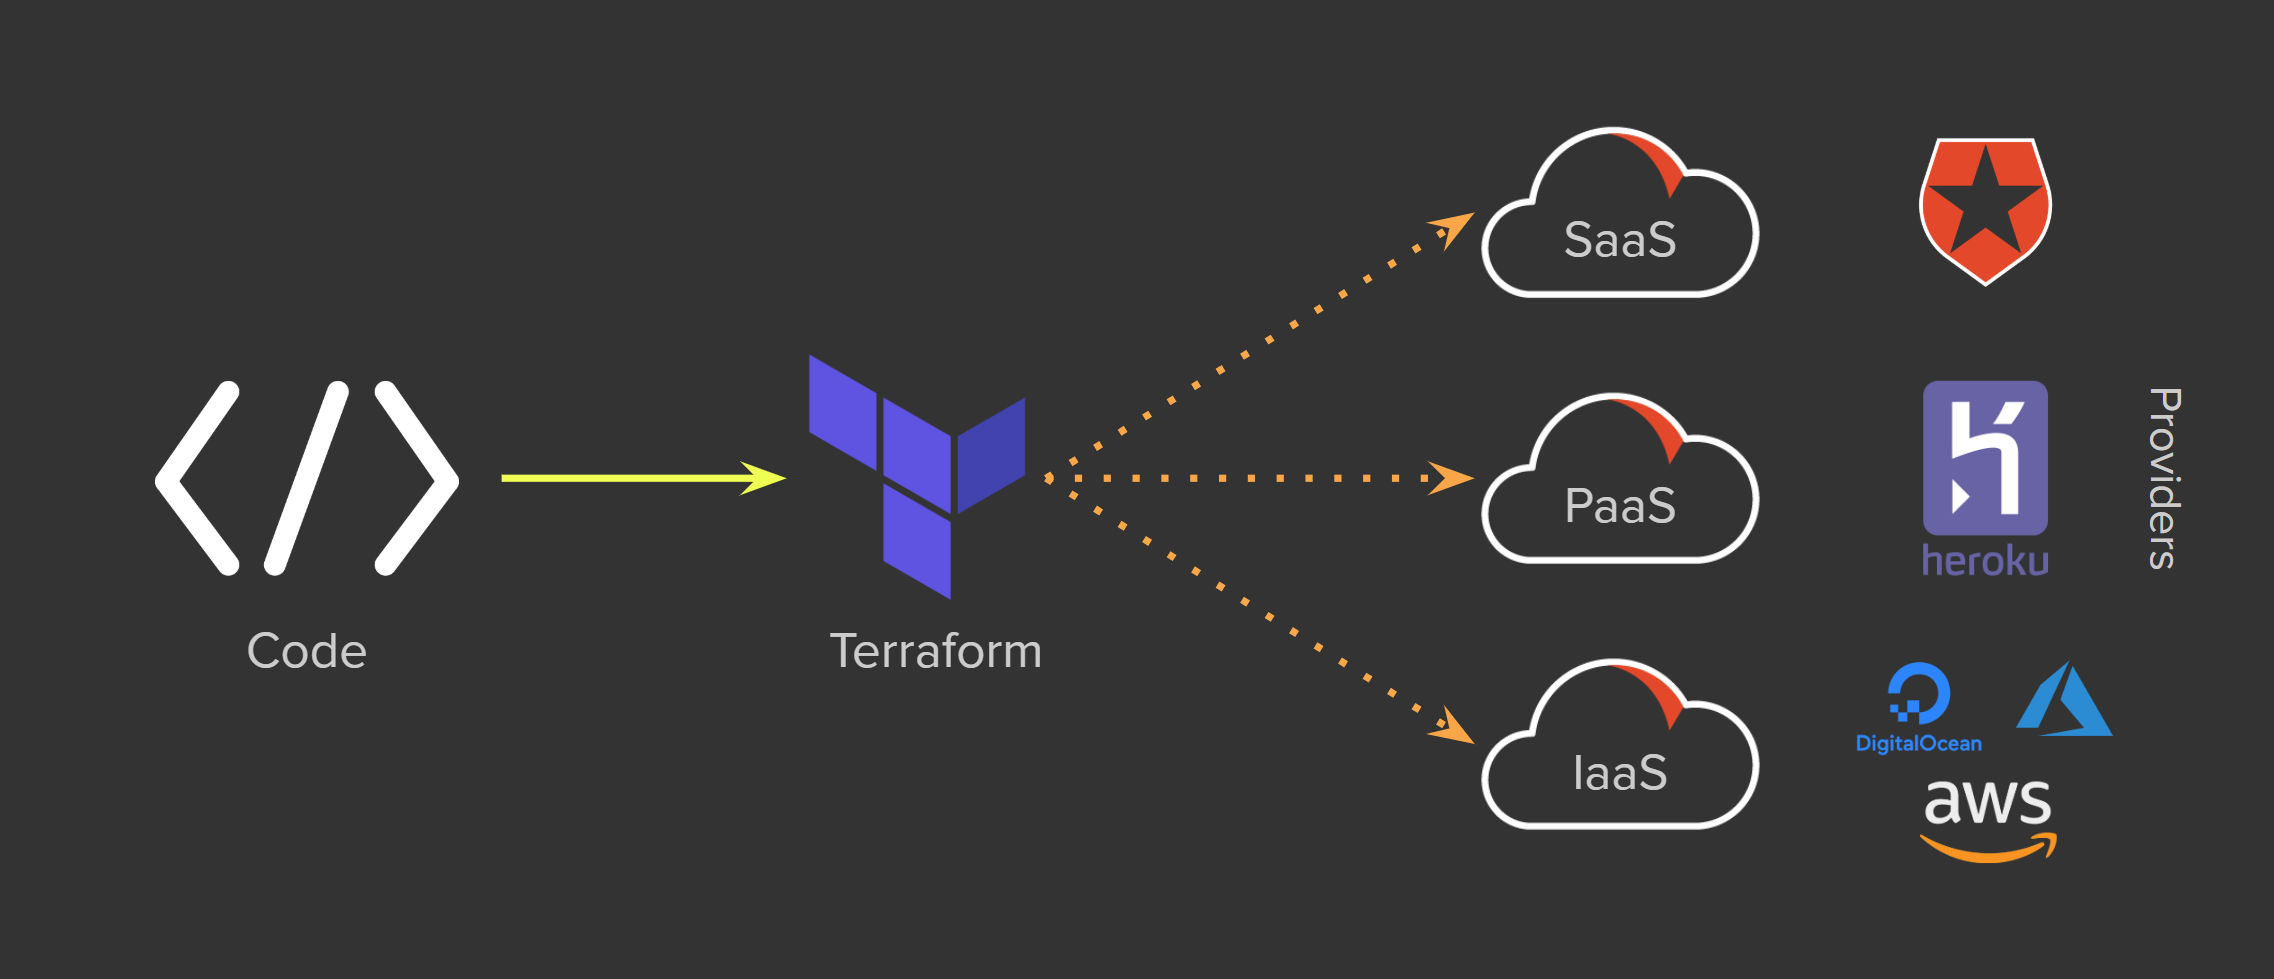
\includegraphics[width=1.0\textwidth]{terraform}
    \caption{Raffigurazione di come Terraform possa essere usato con diversi tipi di servizi e differenti provider. \cite{terraformimg}}
    \label{fig:terraform}
\end{figure}
\subsection{Jenkins}
Questo è stato uno strumento fondamentale ai fini del progetto, nonché ponte di collegamento tra tutte le tecnologie introdotte finora. \\
È un software open source di supporto allo sviluppo che permette facilmente l'integrazione continua e automatica nei rilasci del software.\cite{jenkins}\\
Jenkins è stato utilizzato in questo progetto per costruire delle cosiddette pipeline, ovvero delle collezioni di eventi che succedono uno dopo l'altro. 
In ogni pipeline prodotta vi sono quindi diversi blocchi di azioni che vengono eseguite tramite appositi script scritti in Bash. \\
Ogni qualvolta viene fatta una modifica, un trigger viene attiva e una pipeline specifica viene eseguita in autonomia e senza bisogno di passi manuali. \\ \\ \\ \\ \\ \\ \\
\begin{figure}[h]
	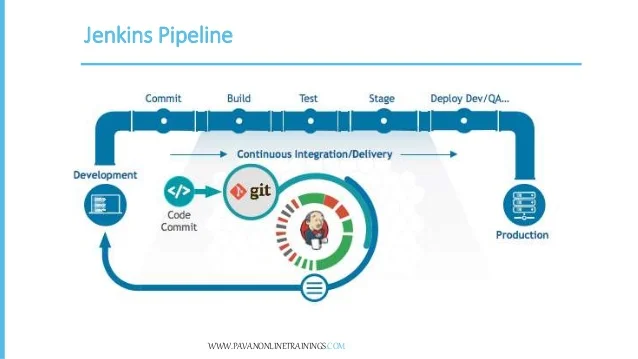
\includegraphics[width=1.0\textwidth]{jenkins}
    \caption{Rappresentazione grafica di una pipeline eseguita da Jenkins. \cite{jenkinsimg}}
    \label{fig:jenkins}
\end{figure}
\section{Requisiti}
Richiamando in breve i requisiti e analizzandoli, l'infrastruttura finale doveva rispettare le seguenti richieste:\\
\begin{enumerate}
\item \textit{Deve essere realizzata tramite una soluzione IAC.}
\item \textit{Deve essere rilasciata in automatico attraverso il cloud.}
\item \textit{Deve essere in grado di ospitare sopra di essa applicazioni a microservizi.}
\item \textit{Deve garantire che le modifiche a questi microservizi vengano integrate e deployate in automatico.}
\end{enumerate}
\subsection{collegamenti tra le tecnologie}
Si tratta di una delle parti più complesse svolte durante il tirocinio. Essenzialmente è stato un punto di transizione tra la fase di studio e la fase di progettazione.\\
Ora che abbiamo introdotto a sufficienza tutti gli strumenti utilizzati, è necessario collegarli tra loro e farli comunicare correttamente, così da completare metaforicamente un grande puzzle.\\
Ad esempio Terraform, Kubernetes e Azure sono stati collegati tra loro come se fossero un'entità unica. Kubernetes ci fornisce il controllo sui container, Azure un servizio per avere il cluster già pronto e sempre online e Terraform ci permette di creare la risorsa dal cloud scrivendo solo codice. \\
Per concludere e realizzare effettivamente una soluzione di tipo IAC, infine l'utilizzo di Jenkins per definire la pipeline che va a rilasciare in automatico sul cloud l'infrastruttura definita da codice.\\
La difficoltà principale nel fare ciò è stato capire a fondo che ruolo svolgeva ogni tecnologia così da sapere in che modo serviva per far funzionare al meglio lo strumento successivo.
\chapter{Progettazione dell'infrastruttura}
\section{Lavoro svolto e fasi affrontate}
Il lavoro svolto durante la fase di progettazione è stato diviso in diverse fasi distinte.\\
Inizialmente è stata eseguita la definizione e modellazione dei casi d'uso considerandone un sottoinsieme rispetto a quelli potenziali, così da garantire di rimanere entro le tempistiche imposte dal tirocinio.\\
Successivamente, dopo aver compreso il ruolo di ogni attore/tecnologia, è stata modellata e definita la struttura dell'intera infrastruttura sulla base dei casi d'uso considerati. Nell'arco di questa fase progettuale è stato accentrato soprattutto il ruolo delle metodologie DevOps e IAC in modo da averle fissate e integrate. Oltre a ciò sono stati ulreriormente modellati i casi d'uso approfondendo gli eventi che si vedono susseguire e le componenti coinvolte. \\ \\ \\ \\ \\
\section{Casi d'uso}
\begin{figure}[h]
	\centering
	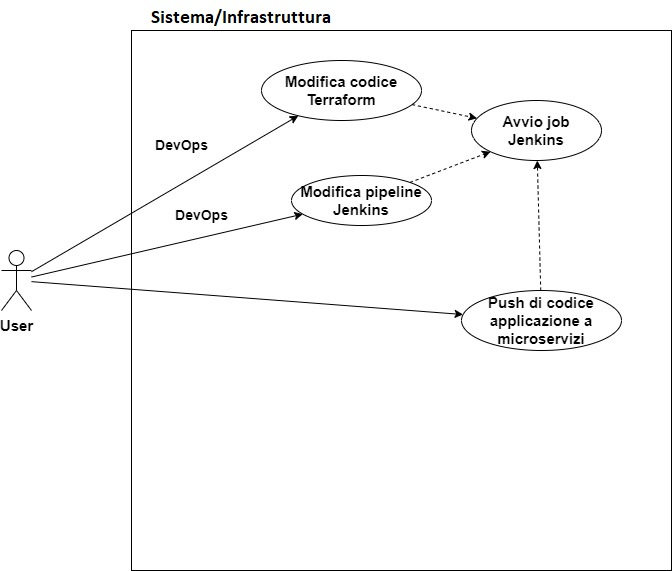
\includegraphics[width=0.7\textwidth]{casi_uso}
    \caption{Diagramma dei casi d'uso considerati in formato UML}
    \label{fig:casi_uso}
\end{figure} 
In figura 7 troviamo il diagramma realizzato in formato UML per rappresentare l'insieme dei casi d'uso considerati nelle fasi preliminari di progettazione.\\
Il sistema è utilizzabile quindi da due tipologie di utenti, chi si occupa della parte DevOps vera e propria e chi invece è lo sviluppatore dell'applicazione a microservizi che andrà ad essere deployata sull'infrastruttura.\\
L'utente DevOps è in grado di eseguire push di eventuali modifiche di codice ai microservizi, ma ha anche i privilegi di amministrazione per modificare il codice lato Terraform o aggiornare delle componenti nelle pipeline. Lo sviluppatore invece può utilizzare l'infrastruttura solo indirettamente eseguendo push di codice innescando i trigger rispettivi. Ognuna di queste azioni attiva uno specifico job jenkins che farà eseguire una pipeline.\\
\subsection{Il ruolo della IAC nel progetto}
Prendendo in considerazione il caso d'uso legato al DevOps, è bene differenziare i concetti legati alla pipeline per il rilascio automatico delle modifiche con approccio DevOps e quella che invece è dedicata alla costruzione IAC. Nel primo caso andiamo a controllare periodicamente entro un certo intervallo di tempo se vi sono state modifiche e in tal caso, vengono integrate e deployate in automatico.\\ Nel secondo caso invece, la pipeline si occupa solamente di eseguire il codice definito in ambito IAC, quindi costruire e rendere operativa l'infrastruttura definita nel sorgente. Eseguendo queste operazioni all'interno di una pipeline dedicata, si ha il vantaggio di non dover fare tutta una serie di azioni in modo manuale, ma di rendere il tutto in automatico. Andando più nel dettaglio, se nel progetto non fosse stata utilizzata questa metodologia e non fosse stata dedicata una pipeline, il processo sarebbe stato il seguente:\\
ipotizzando di non utilizzare Terraform o una tecnologia equivalente, l'alternativa sarebbe stata andare a definire le specifiche direttamente dal portale web del cloud provider scelto o tramite la sua linea di comando dedicata. \\
Anche se a prima vista, il tempo speso per la creazione può sembrare simile, c'è da considerare il tempo che sarebbe speso in una futura manutenzione con eventuali modifiche. In tal caso dovremmo andare manualmente a impartire comandi da linea di comando o dal portale, mentre invece utilizzando una tecnologia di automazione come Terraform, è sufficiente riprendere in mano il codice opportunamente versionato e modificare la componente desiderata.\\
Se adesso consideriamo invece l'utilizzo di Terraform ma senza l'ausilio di una pipeline, anche in questo caso andremmo a investire maggior tempo poiché saremmo costretti manualmente a impartire comandi compilazione e esecuzione del codice scritto, al contrario eseguito in automatico con un'opportuna pipeline definita in primo luogo. \\
\section{Definizione dell'infrastruttura}
\begin{figure}[h]
	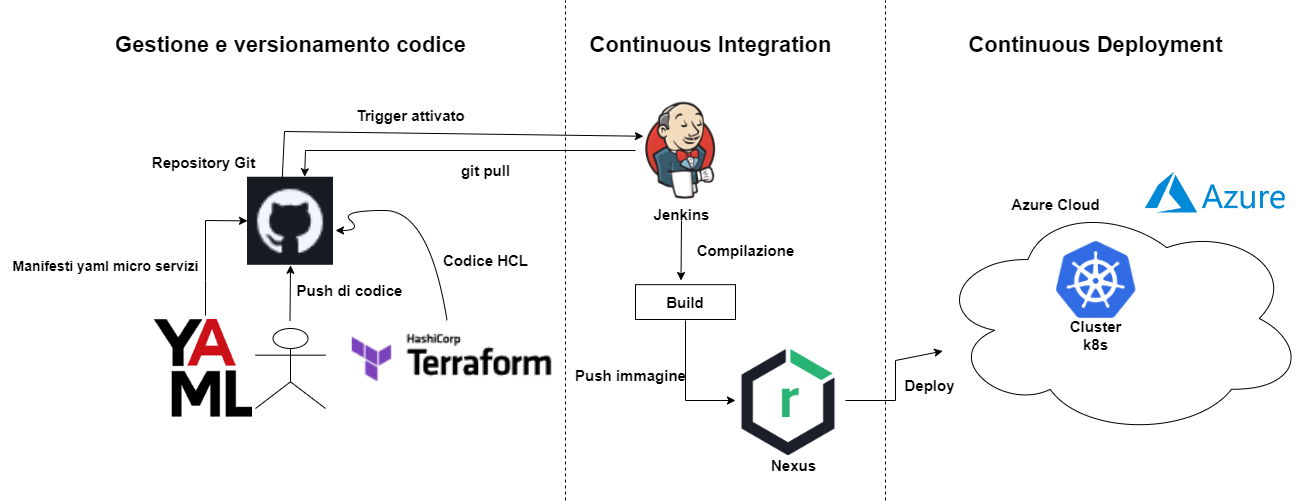
\includegraphics[width=1.0\textwidth]{disegno_struttura_infra}
    \caption{Disegno che definisce il funzionamento dell'intero sistema sviluppato.}
    \label{fig:disegno_struttura_infra}
\end{figure}
In figura 8 è presente il disegno progettuale che definisce la struttura dell'infrastruttura, il quale è stato realizzato successivamente alla modellazione dei casi d'uso considerati. Qui è possibile notare come abbia diviso in tre macro aree la struttura principale del sistema, dalla gestione del codice all'integrazione delle modifiche fino ad arrivare al deploy e resa operativa dei servizi.\\
A partire da sinistra abbiamo tutto ciò che riguarda il versionamento del codice. Alla base vi è un repository Git, il quale può essere quello che contiene il codice Terraform(\textit{e in questo caso specifico spenderemo qualche parola in più nel paragrafo successivo}) oppure uno dei repository che contiene il codice di uno dei microservizi che andranno ad essere deployati sopra il sistema.\\
Per dare più chiarezza sull'utilizzo dei repository dei microservizi, essenzialmente tramite essi è stato preso il codice scritto dallo sviluppatore alla fonte e come prima azione è stato definito all'interno del repository un manifesto in formato YAML per le specifiche del container compatibile con Kubernetes.\\
Nel momento in cui viene eseguito un push sul repository, in particolare sul ramo master, viene attivato un trigger da Jenkins, il quale farà partire l'esecuzione della pipeline collegata.\\
Come prima azione quindi viene eseguito un pull delle modifiche oppure eseguito direttamente il clone dell'intero repository. Successivamente il codice viene compilato, ne viene costruita e versionata l'immagine per il container, poi viene eseguito un push su un repository Docker privato e infine viene eseguito il deploy effettivo sul cluster Kubernetes, utilizzando il manifesto definito in precedenza.\\
Il repository privato per le immagini è stato ospitato tramite Nexus che è una tecnologia dedicata a questo tipo di utilizzo.
\subsection{Ulteriori dettagli progettuali}
Ora che è stato presentato il disegno che rappresenta la definizione completa, andremo a considerare separatamente la modellazione eseguita sui casi d'uso. In particolare consideriamo la casistica in cui viene modificato solo il codice Terraform e quindi la pipeline dedicata allo IAC. Senza ulteriori dettagli invece, avendolo già spiegato, il caso in cui viene applicata una modifica sui microservizi con conseguente deploy. \\  
\begin{figure}[h]
	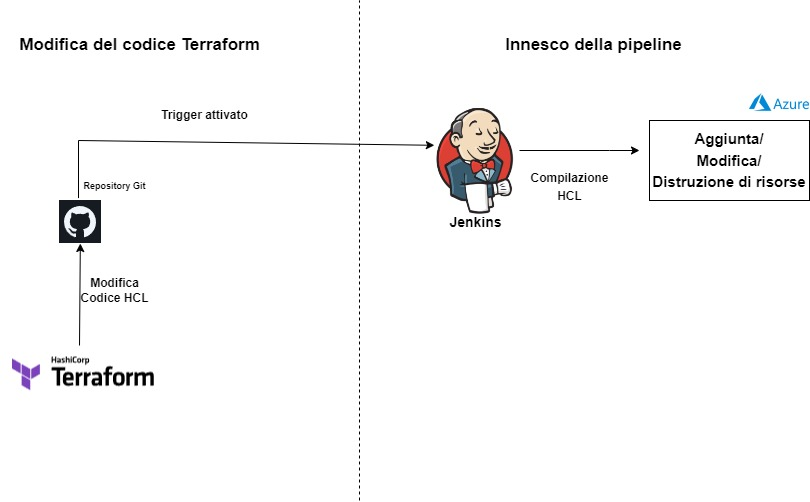
\includegraphics[width=1.0\textwidth]{modifica_terraform}
    \caption{Disegno che rappresenta il caso d'uso della gestione delle modifiche del codice Terraform con l'esecuzione della pipeline IAC.}
    \label{fig:modifica_terraform}
\end{figure} 
\newline In figura 9 vi è un disegno progettuale realizzato per tutto ciò che ruota attorno all'infrastruttura definita come IAC.\\
In questo contesto non stiamo andando a rilasciare delle normali modifiche di microservizi sopra il sistema, ma stiamo considerando l'eventuale modifica dell'infrastruttura stessa definita come codice in termini di soluzione IAC.\\
Nel momento in cui il codice Terraform viene modificato e si verifica un push sul repository, all'interno dell'intervallo di tempo definito, Jenkins attiva il trigger e la pipeline. In questa casistica viene solo eseguito lo script in Bash che va a compilare e eseguire il codice HCL di Terraform, causando l'aggiunta, la modifica oppure la distruzione di risorse.\\
I vantaggi di avere una pipeline dedicata solo per la costruzione o la modifica dell'infrastruttura stessa combinata con l'utilizzo di una tecnologia di automazione come Terraform sono già stati affrontati nel paragrafo 3.2.1. Ma è bene sottolineare nuovamente come senza di essa non sarebbe possibile avere la stessa efficienza in termini di velocità di definizione, costruzione e manutenzione nel lungo periodo.\\
\begin{figure}[h]
	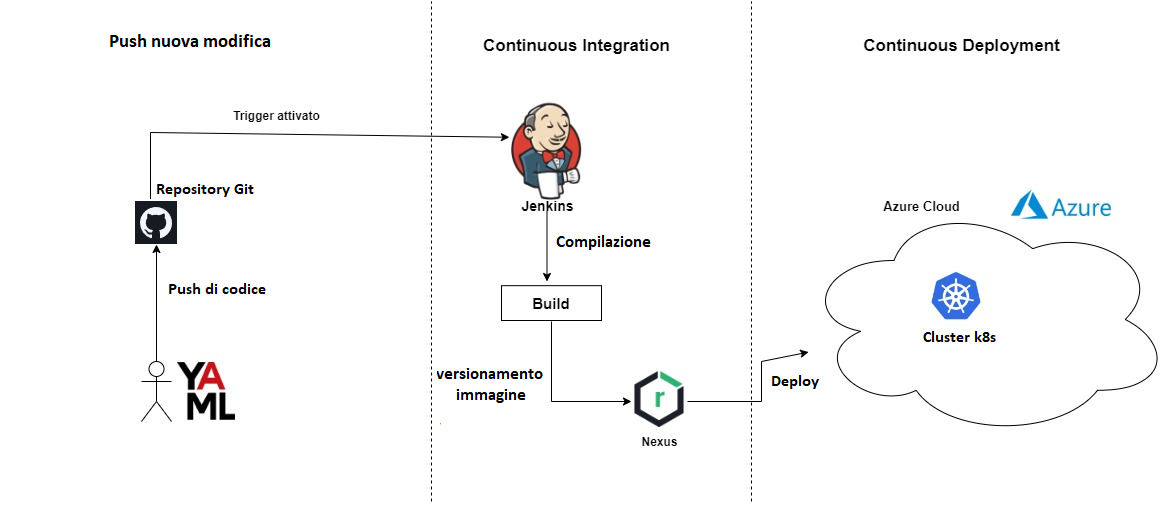
\includegraphics[width=1.0\textwidth]{push_modifica}
    \caption{Dettaglio progettuale per il deploy di nuove modifiche dei microservizi.}
    \label{fig:push_modifica}
\end{figure}
\newline In Figura 10 vi è un disegno progettuale che invece tratta il rilascio automatico delle modifiche dei microservizi deployati sull'infrastruttura. Il processo che va ad eseguire le azioni necessarie per fare ciò è analogo a quanto descritto nel paragrafo 3.2 per la figura 8. Essenzialmente il disegno è molto simile, è stata ignorata tutta la parte IAC e tenuto conto solo delle pipeline di rilascio in ambito DevOps.\\
\chapter{Implementazione dell'infrastruttura}
\section{Codice Terraform e pipeline dedicata}
La fase di implementazione, sulla base del sistema progettato descritto nel capitolo precedente, è iniziata costruendo prima l'ambiente operativo di sviluppo. \\
Per fare ciò è stato prima prodotto il codice Terraform e successivamente sviluppata la pipeline dedicata al rilascio delle modifiche di tale codice.
\subsection{Definizione via codice}
All'interno dei sorgenti HCL sono state definite le specifiche che doveva avere il cluster Kubernetes di Azure. Nel dettaglio è stato deciso di quanti nodi si doveva comporre, la dimensione delle macchine e il numero massimo di pod che poteva sostenere ogni nodo. \\Inoltre è stata definita una risorsa locale di tipo stringa per generare un suffisso casuale in modo da evitare conflitti con eventuali risorse di nome identico già presenti sul cloud.\\
È stato impostato l'autoscale sui nodi con un minimo di tre fino a un massimo di sei. Il numero massimo di pod è stato impostato a 30.\\
Il numero di nodi e di pods è stato scelto in funzione dell'eventuale carico a cui poteva essere sottoposto il sistema. In questo contesto l'applicazione finale che doveva essere rilasciata aveva solamente 4 microservizi e il suo scopo era di elaborare e gestire dei quiz da colloquio tecnico aziendale. Ipotizzando un utilizzo non intensivo è stato ragionevole scegliere un basso numero di nodi a garantire che l'applicazione fosse online anche nel caso in cui uno di essi fosse andato offline, mentre il numero di pods era più che sufficiente a gestire il numero di eventuali repliche da distribuire sui tre nodi.\\
Le informazioni relative al gruppo risorse e la regione geografica sono impostate come variabili all'interno di un altro sorgente e possono essere richiamate tramite il prefisso \textit{'var'}. In questo modo se dovesse essere necessario modificare questi valori, non andrò a toccare il sorgente main, ma cambierò solo le variabili contenute nel sorgente dedicato, così da rendere più mantenibile tutto il codice.\\
Allo stesso modo vi è un file sorgente chiamato \textit{'output'} atto a contenere tutte quelle informazioni che si intende recuperare rapidamente una volta creata e deployata la risorsa definita. In questo caso sono stati scelti i valori relativi al gruppo risorse e al nome del cluster creato, così da reperirli con un apposito comando.\\
Un'ulteriore file \textit{provider} è necessario per definire e comunicare all'interprete quale provider intendiamo utilizzare in modo che durante l'inizializzazione dell'ambiente vengano installate le componenti necessarie a far eseguire il codice correttamente. Dunque in questo caso essendo Azure il nostro fornitore di servizi, si va a specificarlo in questo file dedicato, svolgendo un'operazione simile a un'importazione di libreria per un linguaggio standard.\\
È a questo punto che è possibile toccare con mano tutti i vantaggi della metodologia IAC descritti nei capitoli precedenti. È stato possibile definire e costruire l'infrastruttura senza ausilio di hardware fisico, ma solamente progettandola a un livello alto d'astrazione e realizzandola con il solo uso di codice e oggetti astratti.\\
Qui di seguito può essere visionato il sorgente prodotto per il file main così da apprendere meglio la struttura del linguaggio dichiarativo implementato da Terraform e come nel dettaglio viene definita una risorsa e le sue specifiche.\\ \\ \\ 
\begin{lstlisting}[caption={\\\textit{Codice sorgente all'interno del file main.tf prodotto.\\ }}]
#Definizione della risorsa di tipo cluster Kubernetes
resource "azurerm_kubernetes_cluster" "k8s" {
  name                = "k8s-cluster-iac-${random_string.suffix.result}"
  location            = var.resource_group_location
  resource_group_name = var.resource_group_name
  dns_prefix          = "aks-dns"

  default_node_pool {
    name                = "agent"
    node_count          = 3
    vm_size             = "Standard_DS2_v2"
    max_pods            = 30
    enable_auto_scaling = true
    min_count           = 3
    max_count           = 6
  }

  identity {
    type = "SystemAssigned"
  }
  depends_on = [
    random_string.suffix
  ]
}

#risorsa di tipo stringa per generare il suffisso di 3 caratteri casuali sul nome della risorsa
resource "random_string" "suffix" {
  length  = 3
  special = false
} 
\end{lstlisting}
\subsection{Pipeline per la gestione delle modifiche}
La pipeline è stata divisa in 3 job diversi:\\
\begin{enumerate}
\item \textit{Git clone.} \\
Il primo passo fa semplicemente il clone del repository previo cancellazione della workspace directory per un clone pulito.\\
L'eliminazione della cartella di lavoro è una scelta fatta spuntando un'apposita flag e risulta conveniente per assicurarsi che ogni volta venga eseguito un clone pulito di tutto il progetto onde evitare eventuali conflitti con file residui precedenti.\\
\textbf{Jenkins} fa partire questo primo job solo in caso di modifiche apportate lato \textbf{Git} e effettua un controllo per verificarlo ogni 15 minuti tramite un cronjob definito tramite l'interfaccia web. \\
L'intervallo di tempo scelto per eseguire un controllo sulle modifiche è stata una scelta di progetto. Se si fosse scelto di eseguirlo ogni minuto, in questo contesto specifico non ci sarebbero cambiamenti significativi avendo pochi servizi, ma nel caso in cui così non fosse, le prestazioni della macchina su cui è installato Jenkins ne risentirebbero. \\In un caso estremo avremmo che tutte le pipeline andrebbero in esecuzione contemporaneamente, causando un'eventuale esaurimento delle risorse computazionali e problemi nel rilascio. \\
Dunque, per simulare una situazione reale, è stato scelto 15 minuti per avere la certezza di più rilasci nell'arco della giornata e minimizzando la probabilità di avere tutte le pipeline in esecuzione nello stesso momento.\\ \\ \\ \\ \\
\item \textit{Build Terraform.} \\
In questo passo intermedio viene effettuato un login su Azure per assicurarsi di essere autenticati con la sottoscrizione corretta. In questo modo se la macchina dovesse essere utilizzata anche da altri utenti si evita di andare a fare modifiche su macchine che risiedono su altre sottoscrizioni Azure controllate da altri DevOps.\\
Fatto questo, viene effettuata la compilazione del codice e applicato allo stesso tempo, eseguendo eventualmente le azioni necessarie a modificare l'infrastruttura.\\
La scelta di un passo intermedio prima del deploy effettivo è dovuta all'eventualità di errori nel codice, così da bloccare preventivamente la pipeline senza passare al blocco successivo.\\
\item \textit{Deploy test.} \\
In questo ultimo passo viene semplicemente testato che il cluster Kubernetes sia stato creato correttamente e che sia funzionante, rilasciando sopra di esso una piccola applicazione di test.\\
Anche questa è stata una scelta presa durante lo sviluppo, poiché se questa applicazione minimale risulta attiva sul cluster, è garantito che il sistema stia funzionando correttamente dopo essere stato deployato nel passo precedente.
Come già detto se il job relativo alla build del codice non viene concluso correttamente senza errori, la pipeline si ferma senza far cominciare quest'ultimo.\\
Questo accade per ogni concatenazione, avendo impostato tramite un apposito flag che i trigger di post-compilazione si attivano solo se la compilazione del processo attualmente in esecuzione è stabile.\\ \\ \\ \\ \\ \\
\end{enumerate}
Le credenziali di accesso sono gestite tramite un sistema interno di \textbf{Jenkins} dove è possibile definirle comodamente per poi utilizzarle come variabili negli script \textbf{Bash}.\\
Inoltre, per tenere traccia delle risorse attualmente attive, \textbf{Terraform} crea durante la prima esecuzione del codice un file di configurazione dello stato corrente, il quale viene aggiornato di volta in volta. In questo modo se si esegue due volte lo stesso codice, non viene creata due volte la risorsa.
\begin{lstlisting}[caption={\\\textit{Frammento di codice relativo alla compilazione del codice Terraform.\\ Nelle ultime righe viene effettuato un collegamento con il cluster appena creato e lanciato un comando per visualizzare i nodi in modo da accertarsi che sia operativo.}}]
az login -u $azure_user -p $azure_psw
terraform init
terraform apply -auto-approve 

rs_group=$(terraform output resource_group_name | cut -d '"' -f 2)
cluster_name=$(terraform output kubernetes_cluster_name | cut -d '"' -f 2)
az aks get-credentials --resource-group $rs_group --name $cluster_name
kubectl get nodes
\end{lstlisting}
\section{Sviluppo pipeline per il rilascio dei micro servizi e modifica di puntamenti nel sorgente}
Una volta definita e resa operativa l'infrastruttura progettata, è stato possibile in una seconda fase di implementazione andare a eseguire il rilascio dell'applicazione a microservizi citata in precedenza come test conclusivo del funzionamento del sistema e del rispetto dei requisiti del progetto. \\ \\ \\
\subsection{Definizione delle pipeline}
L'applicazione, oltre ai suoi quattro microservizi, comprendeva anche il frontend e un api gateway. Per ognuna di queste componenti è stata sviluppata una pipeline dedicata.\\
In questo modo anche la gestione delle modifiche di ogni servizio è indipendente e isolata come i microservizi stessi. Questo va a garantire che nel momento in cui avviene un push su un repository, si vada a integrare solamente quelle modifiche senza intaccare il resto delle componenti dell'applicazione rimaste invariate.\\ \\
Ogni pipeline era composta dai seguenti job singoli:\\
\begin{enumerate}
\item \textit{Git clone.}\\
Senza ripetersi, svolge un'azione identica al primo passo della pipeline per il codice Terraform.\\
\item \textit{Build codice.}\\
In questo step viene solamente compilato il codice in locale. Se non ci sono errori, si passa alla build dell'immagine Docker.\\
Come per la pipeline relativa al codice Terraform, è stato scelto di inserire un passo intermedio per la compilazione del codice così da bloccare il processo subito in questo punto nel caso vi siano errori rilevati nel codice o di altra natura.\\
\item \textit{Build immagine.}\\
Prima di tutto viene eseguito il login sul repository Docker privato. Questo per far si che le prossime operazioni vengano eseguite sul nostro repository e non su un altro ipoteticamente utilizzato da un altro utente DevOps che ha accesso alla nostra stessa macchina. Successivamente a partire dal codice già compilato viene eseguita la build dell'immagine usando il relativo Dockerfile presente nel repository clonato. Oltre a ciò viene anche eseguito il versionamento dell'immagine in modo da poter effetuare eventuali rollback in futuro.\\
L'uso di un repository privato per le immagini Docker garantisce che anch'esse siano confidenziali e non accessibili pubblicamente, oltre al codice che è già contenuto all'interno di repository privati.\\
\item \textit{Deploy k8s.}\\
In quest'ultimo passo viene anche qui eseguito un login su Azure, ci si collega al cluster corretto e infine viene applicato il manifesto YAML presente sul repository.\\
In particolare al primo deploy, viene semplicemente applicato il manifesto e creati i container. Per quanto riguarda invece il successivo rilascio delle modifiche, viene sfruttato il meccanismo di Kubernetes citato in precedenza facendo si che con un apposito comando, venga prima creato il container che utilizza l'immagine aggiornata e solo infine terminare il container vecchio.\\
Facendo così, l'utente finale non avrà mai problemi di downtime durante l'utilizzo dell'applicazione, semplicemente ad un certo punto si ritroverà una nuova versione in tempo reale. \\ \\ \\ \\ \\ \\ \\ \\ \\ \\ \\ \\
\end{enumerate}
\begin{lstlisting}[caption={\\\textit{Frammento di codice relativo al versionamento e alla build dell'immagine.}}]
#login sul repository docker
sudo docker login -u $docker_usr -p $docker_psw http://localhost:8083/repository/docker-hosted/
#Build dell'immagine dal Dockerfile(prelevo ultimo numero di versione dal repo docker)
img=interview_quiz
version=$(sudo docker images localhost:8083/repository/docker-hosted/interview_quiz --format "{{.Tag}}" | grep -A 1 latest | awk 'NR==2')
if [ -z "$version" ]; then
	version="v1"
else
    #estraggo il numero di versione e lo incremento di 1
    version_number=$(echo "$version" | cut -c 2-)
    new_version_number=$((version_number + 1))
    version="v$new_version_number"
fi
sudo docker build -t $img .
\end{lstlisting} 
\begin{figure}[h]
	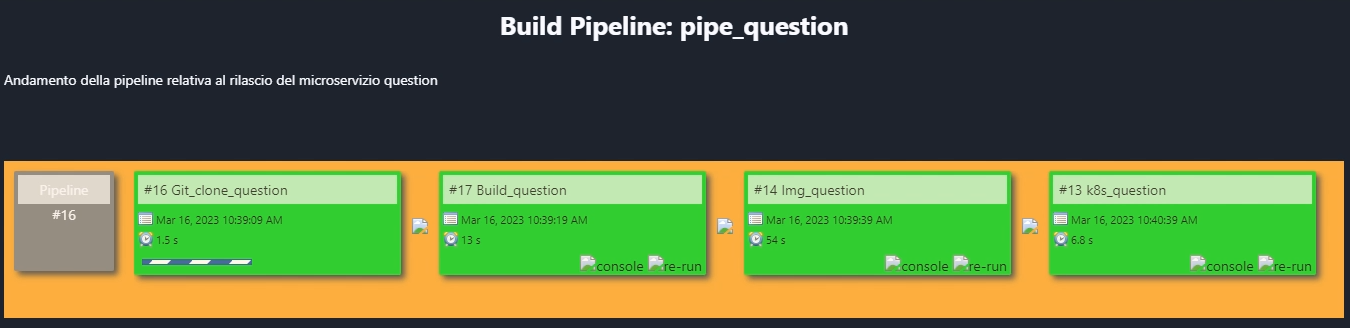
\includegraphics[width=1.0\textwidth]{pipeline}
    \caption{Una delle pipeline sviluppate per il rilascio automatico delle modifiche di un microservizio.}
    \label{fig:pipeline}
\end{figure}

In figura 11 è possibile vedere una delle pipeline sviluppate attraverso l'interfaccia grafica web di Jenkins. Come descritto nel paragrafo 4.2.1, ognuna di esse è stata sviluppata in modo da avere 4 job distinti che vengono avviati in successione se l'esecuzione del job precedente viene conclusa con successo. Da sinistra si inizia con il clone del repository fino ad arrivare a destra nell'ultimo processo, il quale provvede a deployare e concludere l'esecuzione dell'intera pipeline.\\
\subsection{Modifica nel codice sorgente}
Dopo aver sviluppato le pipeline, per poter rendere l'applicazione già sviluppata compatibile con il sistema finora costruito, si è reso necessario apportare alcune piccole modifiche ai puntamenti presenti nel codice sorgente.\\
All'interno del servizio api gateway, sono state modificate tutte le rotte mettendo al loro posto il nome di dominio FQDN di ogni servizio definito nei manifesti per Kubernetes. Ad esempio se il microservizio si chiama \textit{question} ed è stato esposto sulla porta 8082, nella rotta viene inserito: \textit{http://question-service.interview-tool.svc.cluster.local:8082}\\ \\
Per come era strutturata l'applicazione architetturalmente, solo il frontend e l'api gateway sono stati esposti su internet, mentre i quattro microservizi comunicavano tra loro internamente al cluster ed erano raggiungibili dall'esterno solamente passando attraverso il gateway.\\
Qui di seguito ho posizionato uno dei manifesti in formato YAML definito per uno dei quattro microservizi chiamato user.\\ 
Nella prima parte è definito un oggetto di tipo deployment che presenta le specifiche del container, a partire dal nome, namespace fino all'immagine che dovrà esserci montata sopra.\\ 
Sempre sul deployment sono stati definiti anche dei volumi per montare delle chiavi necessarie per il microservizio, oltre a delle variabili d'ambiente per richiamare il database.\\ 
Nella seconda parte del manifesto è definito un oggetto di tipo service per esporre sulla porta 8080. \\ \\ \\ \\ \\ \\
\begin{lstlisting}[caption={\\\textit{Il manifesto YAML appena citato e descritto.}}]
apiVersion: apps/v1
kind: Deployment
metadata:
  name: user-deployment
  namespace: interview-tool
  annotations:
    meta.version: "v1"
  labels:
    app: user
spec:
  replicas: 1
  selector:
    matchLabels:
      app: user
  template:
    metadata:
      labels:
        app: user
    spec:
      imagePullSecrets:
      - name: regcred
      containers:
      - name: user
        image: <nome-immagine>
        imagePullPolicy: Always
        ports:
        - containerPort: 8080
        volumeMounts:
        - mountPath: /certificates/public/
          name: public-pem
        - mountPath: /certificates/private/
          name: private-pem
        env:
        - name: MYSQL_HOST
          value: db-user-service
        - name: MYSQL_USER
          value: root
        - name: MYSQL_PASSWORD
          value: password
      volumes:
      - name: public-pem
        secret:
          secretName: public-key
      - name: private-pem
        secret:
          secretName: private-key        
---
apiVersion: v1
kind: Service
metadata:
  name: user-service
  namespace: interview-tool
spec:
  selector:
    app: user
  ports:
  - name: user-service
    port: 8080
    targetPort: 8080
\end{lstlisting}
Un'ulteriore modifica è stata effettuata ai file di proprietà di ogni microservizio per regolare le rotte interne al cluster, sempre utilizzando il nome dominio FQDN dei servizi come fatto nel gateway. Sempre negli stessi file è stata modificata la rotta per il collegamento al database in modo da far collegare il microservizio al container del database definito tramite Kubernetes.\\
In questo modo, l'applicazione che prima era stata definita per essere eseguita e testata in un ambiente locale, ora ha le caratteristiche necessarie per essere eseguita sul cloud all'interno del cluster Kubernetes definito. \\ \\ 
Giunti a questo punto, il sistema risulta completo, dunque se lo sviluppatore di questa applicazione dovesse apportare delle modifiche a uno qualunque dei microservizi che la compongono, verrebbero deployate in tempo reale nell'arco di 15 minuti totalmente in automatico seguendo le procedure descritte nei precedenti paragrafi. \\
L'unico aspetto manuale che è doveroso considerare rientrerebbe nel caso in cui si volesse fare rollback a una versione precedente. In tal caso sarebbe necessario eseguire un comando dalla CLI di Kubernetes specificando la versione dell'immagine di cui eseguire il pull, creando così il nuovo container e eliminando quello basato sull'immagine contenente eventuali problemi. \\ \\ \\ \\ \\ \\ \\  
\begin{figure}[h]
	
\includegraphics[width=1.0\textwidth]{app_micro}
    \caption{Schermata principale dell'applicazione una volta deployata con successo sull'infrastruttura sviluppata.}
    \label{fig:app_micro}
\end{figure}
\begin{figure}[h]
	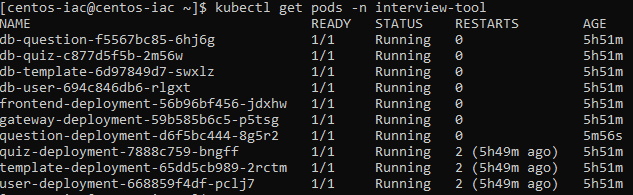
\includegraphics[width=1.0\textwidth]{app_micro2}
    \caption{Visualizzazione dei container in esecuzione per l'applicazione rilasciata nel suo namespace specifico. \\Ogni microservizio ha un suo database indipendente.}
    \label{fig:app_micro2}
\end{figure}
\begin{figure}[h]
	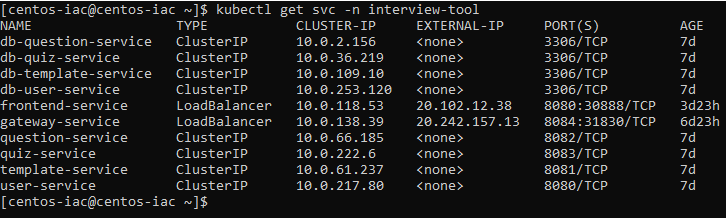
\includegraphics[width=1.0\textwidth]{app_micro3}
    \caption{Visualizzazione di tutti i servizi attivi per l'applicazione rilasciata.\\Come spiegato in precedenza, abbiamo solo due servizi esposti su internet, mentre gli altri 4 comunicano internamente al cluster e sono raggiungibili attraverso il gateway.}
    \label{fig:app_micro3}
\end{figure} \leavevmode \\ \\ \\ \\ \\ \\ \\ \\ \\ \\ \\ \\ \\ 
\section{Problemi incontrati lungo il progetto e approcci utilizzati}
Durante lo sviluppo del progetto sono stati incontrati diversi problemi, i quali sono stati affrontati con determinati approcci per risolverli e/o deviarli.\\ \\
\begin{itemize}
\item \textit{\textbf{Fase di studio.}}\\
Nella fase di studio, come accennato anche in precedenza, il problema maggiore è stato comprendere il ruolo di ogni strumento nel contesto specifico in cui dovevano essere utilizzati. Questo ha fatto si che la fase iniziale di studio sia stata lenta per poi gradualmente accelerare verso la sua fine.\\
L'approccio standard numero uno è stato leggere buona parte della documentazione ufficiale per capire i funzionamenti, eventualmente integrando queste informazioni sfruttando risorse sul web come ad esempio video molto approfonditi su YouTube.\cite{youtubek8s}\\
Man mano che le tecnologie viste e i concetti aumentavano, il modo più efficiente per cercare di tenere il tutto coeso ed evitare confusione è stato continuare a farsi determinate domande come ad esempio: \\ \textit{Se con Docker posso creare e gestire container, ma con Kubernetes posso fare lo stesso, qual è la differenza fondamentale?} \\ \textit{Ora che so che su Azure c'è un servizio che mi garantisce un cluster Kubernetes pronto e operativo, come posso fare per definirlo, modificarlo o cancellarlo in automatico rispettando i requisiti?} \\ \\ \\ \\ \\
\item \textit{\textbf{Fase di progettazione.}}\\
In questa fase l'unica difficoltà è stata definire accuratamente i casi d'uso da implementare successivamente ed eventualmente escluderne altri.\\
L'approccio è stato intuitivamente andare ad analizzare i requisiti iniziali e da essi esportare i possibili casi d'uso che potevano verificarsi sul sistema, ovvero quelli mostrati nel capitolo 3 in figura 7. Nel resto della progettazione non vi sono state ulteriori criticità considerando la chiarezza dei requisiti ed essendo appena usciti dalla fase di studio con tutti i concetti carpiti.\\
\item \textit{\textbf{Fase di implementazione.}}\\
Inizialmente, vi è stata una scelta di implementazione per quanto riguarda il tipo di oggetto con cui sviluppare le molteplici pipeline.\\
In \textbf{Jenkins} ci sono diversi modi per lavorare con le pipeline e un primo approccio utilizzato durante la fase di studio per poi testarlo in sede di implementazione è stato l'uso di uno script adibito a pipeline. Questo metodo di sviluppo è molto potente siccome è possibile definire tutti i vari blocchi in uno script unico all'interno di un file che verrà chiamato Jenkinsfile. Tuttavia, dovendo simulare una situazione reale, risulta difficile da mantenere all'interno di un team più ampio avendo più utenti che ci devono mettere le mani sopra.\\
Dunque a risoluzione di questo problema è stato optato invece l'utilizzo di diversi progetti detti freestyle, ovvero dei job singoli ognuno con il proprio contenuti di azioni come descritto nel capitolo 4, allegando poi dei trigger di post-compilazione per regolare quale evento succede l'altro.\\
Durante la fase finale di rilascio, una delle difficoltà è stata il dover prendere in carico il codice di un'applicazione scritto da un'altra persona. In un primo momento c'è stata la nacessità quindi di comunicazione per avere una panoramica sulla struttura architetturale dell'applicazione, così da avere un'idea più precisa di come i microservizi comunicassero tra di loro a livello tecnico. In un secondo momento invece è stata approfondita in autonomia la struttura osservando i vari repository per comprendere il punto esatto in cui si rendeva necessaria la modifica delle rotte e i relativi puntamenti. Pur non avendo conoscenze approfondite degli strumenti di utilizzati dallo sviluppatore, in seguito all'analisi del sorgente è stato possibile ricavare dove effettuare le modifiche, adattandole poi con le diciture definite nei manifesti YAML scritti in precedenza.\\
Un ulteriore problema riscontrato è stato quello di combinare la tecnologia \textbf{Nexus} con il cluster \textbf{Kubernetes}.\\
Qui affrontiamo direttamente lo svantaggio dell'utilizzo di un servizio preconfezionato quale è \textbf{AKS(Azure Kubernetes Service)}. La criticità principale risiedeva nel fatto che il pull delle immagini da parte del cluster avveniva obbligatoriamente attraverso il protocollo HTTPS, mentre il repository ospitato su Nexus come opzione di default viaggiava in HTTP.\\
Un primo approccio è stato quello di provare a forzare l'AKS a eseguire il pull mediante registro non sicuro, ma è stato abbastanza chiaro capire che questo non era possibile.\\
Un secondo approccio è stato creare un certificato self-signed da applicare sul repository Docker così che fosse raggiungibile via HTTPS. Nonostante ciò, per come era preconfigurato il cluster, non c'era modo di farsi dare la fiducia su quel certificato al container runtime in esecuzione sotto \textbf{AKS}.\\
Possiamo dire che i vantaggi di un servizio di questo genere sono andati a discapito di un eventuale bisogno di dover modificare la configurazione delle macchine.\\
Ad esempio su un cluster Kubernetes nativo, una semplice soluzione poteva essere andare a modificare la configurazione di ogni nodo in modo che tutti si fidassero di tale certificato.\\
Una volta aggirato l'ostacolo mediante l'uso di un normalissimo repository su Docker Hub, il resto dell'implementazione del sistema non ha avuto altre criticità rilevanti.\\ \\ \\ \\
\end{itemize}
\chapter{Conclusioni}
\section{risultati raggiunti al termine}
Al termine di questo progetto i risultati raggiunti sono stati diversi, li ritroviamo qui di seguito:\\
\begin{itemize}
\item \textit{Appreso competenze in ambito DevOps.}\\
Nel corso del tirocinio è stato possibile approcciarsi da zero con questa metodologia di sviluppo, riuscendo a carpirne i vantaggi del suo utilizzo e a sviluppare nuove competenze.\\
\item \textit{Appreso conoscenze su diverse tecnologie.}\\
Grazie a questo progetto è stato possibile conoscere e acquisire competenze su molte tecnologie in breve tempo. In aggiunta al background accademico, tutto ciò ha arricchito molto il bagaglio di competenze informatiche.\\
\item \textit{Realizzata un'infrastruttura fedele ai requisiti iniziali.}\\
Terminato il progetto, è stata realizzata un'infrastruttura che rispetta i requisiti e i vincoli imposti nel corso del tirocinio, seppur con piccole modifiche rispetto a quanto fatto in sede di progettazione.\\
Come accennato e approfondito al termine del capitolo 4, durante la fase di implementazione è stato reso necessario il non utilizzo di Nexus per il repository Docker privato a causa di ostacoli tecnici deviando quindi su un normale Docker Hub privato per non sforare con i tempi.
\end{itemize}
\section{miglioramenti}
Per quanto riguarda eventuali miglioramenti futuri, ciò che si potrebbe aggiungere è un sistema di monitoraggio dell'intero sistema. Allo stato attuale il controllo e la gestione delle risorse viene eseguito manualmente da shell, ma si potrebbe invece implementare un sistema più sofisticato utilizzando qualche tool esterno come ad esempio Grafana.\\
Un'ulteriore modifica può essere fatta per quanto riguarda la scelta del cloud provider, così da approfondire le differenze tra i diversi servizi e verificare se gli stessi problemi riscontrati in questo contesto, possono essere evitati o meno.
%
%			BIBLIOGRAFIA
%
\begin{thebibliography}{00}
%

\bibitem{certimeter}
Certimetergroup, chi siamo. \url{https://www.certimetergroup.com/chi-siamo}

\bibitem{defdevops}
Wikipedia, DevOps. \url{https://it.wikipedia.org/wiki/DevOps}

\bibitem{cloud}
Ionos.it, I vantaggi del cloud computing. 2023 \url{https://www.ionos.it/digitalguide/server/know-how/i-vantaggi-del-cloud-computing/}


\bibitem{iacdef}
Wikipedia, Infrastructure As Code. \url{https://it.wikipedia.org/wiki/Infrastructure_as_Code}

\bibitem{iaceng}
Wikipedia, Infrastructure as code(iaC). \url{https://en.wikipedia.org/wiki/Infrastructure_as_code#Relationship_to_DevOps}

\bibitem{devopsloopimg}
Shalb, What is DevOps and where is it applied? 2019.\url{https://shalb.com/blog/what-is-devops-and-where-is-it-applied/}


\bibitem{devopsloop}
TechTarget, Demystify the DevOps process, step by step, 2023. \url{https://www.techtarget.com/searchitoperations/tip/Demystify-the-DevOps-process-step-by-step}

\bibitem{docker}
Wikipedia, Docker. \url{https://it.wikipedia.org/wiki/Docker#Orchestrazione}

\bibitem{dockerimg}
Mindmajix, Docker Container Software And Architecture, 2023. \url{https://mindmajix.com/docker-architecture}

\bibitem{kubernetes}
Wikipedia, Kubernetes. \url{https://it.wikipedia.org/wiki/Kubernetes}

\bibitem{k8simg}
Datafusionspecialists, Containerization and Cloud Mobility, 2019. \url{https://datafusionspecialists.com/solutions/containerization-and-cloud-mobility/}

\bibitem{terraformimg}
Auth0, Community Developer Brings HashiCorp Terraform to Auth0, 2020. \url{https://auth0.com/blog/community-developer-brings-hashicorp-terraform-to-auth0/}

\bibitem{jenkins}
Wikipedia, Jenkins. \url{https://it.wikipedia.org/wiki/Jenkins_(software)}

\bibitem{jenkinsimg}
Slideshare, Jenkins Pipeline, 2019. \url{https://www.slideshare.net/pavan5780/jenkins-pipeline-164020728}

\bibitem{youtubek8s}
TechWorld with Nana, Kubernetes for Beginners, 2020. \url{https://www.youtube.com/watch?v=X48VuDVv0do}
%
%
\end{thebibliography}
% 
\end{document}


 
